% Revision information
% $Author$
% $Date$
% $Revision$
%---------------------------------

\documentclass[a4paper]{scrreprt}
\usepackage[pdftex]{graphicx}
\usepackage{geometry}
\geometry{hmargin=2.5cm,vmargin=2.5cm}

\usepackage{lastpage}

%opening
\title{User manual for KipTool\\\vskip30pt
\includegraphics[width=0.4\textwidth]{figures/kip_icon.pdf}}
\author{A. Kaestner}
\begin{document}
\maketitle
\tableofcontents
\chapter{Introduction}
\section{Introduction}
KipTool is a image processing tool mainly intended to process 3D images. It provides a GUI that allows you to load an image from tiff slices and then process it through a chain of processing modules. In 
\chapter{A first example}
KipTool has a number of register tabs for different tasks. In the data part there are four tabs; Project information, Data, Processing
\section{Project information}
The project information tab is used to add information about the current processing task mainly for documentation purposes. You don't have to enter any information here but it can be helpful when you are trying to find out what you did when you return to the data at later time.

\section{Load the data}
To select and load the data you have to provide the full path and file mask in the dedicated field on the top of the data tab. This can be done with help of the browse button which provides a file selection dialog. Navigate to the data and select any file in the data set you want to load and press choose. The correct file mask now appears in the entry field. The file mask is made of a base name (including the path) followed by a number of \#'s to match the file index numbers, \emph{eg.} \verb+slice_####.tif+. KipTool can for the moment only read tiff images. Once you have the file mask you have to select the interval of files using the numeric entries for the first and last image. There is also the possibility to skip files by changing the file increment from 1 to the desired increment number. Now you can press the Load data button and the data is loaded and displayed in the original image viewer. Using the slider below the images you can inspect the loaded data. For this example it is sufficient to load ten slices. 

If the data is too large you can mark a region in the original image viewer and press the ROI button. This will transfer the ROI coordinates to the ROI entries. Now set the check mark for use ROI and then press Load data again to reload the data.
 
\section{Select processing modules}
KipTool works with a set of processing modules that process the image in a sequence. These modules are inserted and configured under the processing tab. When you start KipTool for the first time, the process chain is empty. To add a module press Add to the left in the module configurator, figure \ref{fig_moduleconfigurator}. A file dialog that asks you to select a module library appears, select the AdvancedFilterModules library. 
\begin{figure}[ht!]
\centering
\begin{tabular}{cc}
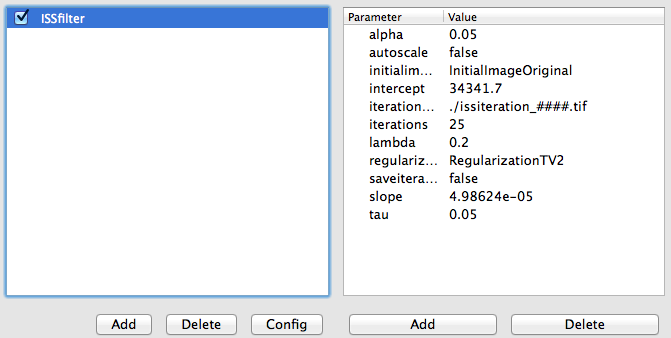
\includegraphics[width=0.6\textwidth]{figures/ModuleConfigurator.png} &
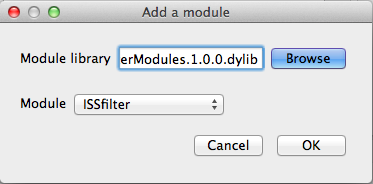
\includegraphics[width=0.3\textwidth]{figures/ModuleSelectionDlg.png} \\
(a) & (b)
\end{tabular}
\caption{The Module configurator (a) and a module selection dialog (b).}
\label{ref_moduleconfigurator}
\end{figure}
Select the ISS filter in the drop-down and press OK. The module now appears in the list to the left in the Module configurator, to the right you see the parameters that are used by the module. You can repeat the add module to insert more modules if you like. If the order of the modules are wrong, you can drag them in the list to rearrange the order.

\section{Start processing and inspect the results}
When the data is loaded and at least one module is configured you can start the processing by going to the Process menu and select Process. The processing starts and when it is completed the result is displayed in the image viewer for processed data. When you now drag the slider below the viewers you can inspect the images in parallel.  

\section{Save the processed data}
When the processing is complete you probably want to save the results to disk. Select the data tab again and enter destination path using the browse button and enter the file mask using \#'s as place holders for the index numbers, exceeding \#'s will be filled with zeros. When you press save the data will be saved in the same format as the original data. You can however also select a different format by using the drop-down for file formats. 

\chapter{Detailed description}
\section{File processing tools}
The file processing tools is a set of tools to process stacks of image without loading all of them into memory. This make them lightweight and puts essentially no resource requirements on the used computer.
\subsection{Reslice}
Reslicing is when you want to permute the image planes of the data. Normally CT is save in the XY plane, perpendicular to the rotation axis. Using this tool you can reslice the data to XZ- and YZ-planes. Reslicing can also be used to build sinograms from a projection data set.

\subsection{Merge volumes}
Extruded samples, i.e. long and narrow, usually don't fit in the field of view. For such samples, it is possible to make several scans while the axis is translated along the acquisition axis with a small overlap. This tool is used merge the reconstructed subvolumes into a single sequence with file indices in a continuous sequence. This essentially a file copy/rename task, except for the overlap region. In this region slices from the two data sets are mixed with sigmoid mixing weight. The weighted mixing guarantees a seamless transition between the data sets.

\subsection{File conversion}
This is mainly a renaming and file type conversion tool. It was originally developed when we had problems with our cameras and a CT scan consisted of several sub-sets. Now it is possible to reshuffle projections acquired with the golden ratio acquisition scheme into a linear sequence. You can also collate images, for the case when several images are acquired at the same angle. The converted images can also be cropped.

\subsection{Generic file conversion}
The generic file conversion is a reverse engineering tool. It is often a hard task to handle  images saved with an unknown/unspecified file format, e.g. dump files from a camera, and want to convert them into something more readable by other software. This tool helps you to identify how data is stored and to save it in a new format.

\section{Processing modules}
There are many modules available for KipTool. Unfortunately many are also under development which means that they can crash the software or are very slow. The modules that are documented here are well tested and will work.
\subsection{The ISS filter}
The Inverse Scale Space Filter is a an edge preserving de-noising filter based on the paper \cite{burger2006}. The filter solves the differential equation:
\begin{eqnarray}
\frac{du}{dt}&=&\frac{\nabla\cdot \nabla u}{|\nabla u|} + \lambda(u-f-v)\nonumber\\
\frac{dv}{dt}&=&\alpha (u-v)
\end{eqnarray}
using an iterative solver on the discrete equations. Here the solution time $T=N\cdot\tau$ can be selected using number of iterations, $N$, and time increments, $\tau$. For stability reasons it is important that the value of $\tau$ is less than 0.125. Decrease $\tau$ if you want to improve the quality of the solution but then $N$ must be increased to maintain constant $T$. The sensitivity to noise is decreased for small $\tau$. Another constraint is that $\alpha<1/4 \lambda$ otherwise the eigenvalues of the system become complex and the solution will oscillate. The equation works best when the data is normalized to zero-mean and variance equal to one, this can be done automatically by setting the parameter autoscale to true. This setting will compute a new normalization for every data set, i.e. if you tune the filter for a small ROI and change to the full image a new normalization will be made and the setting are not guaranteed to be perfect. 
\subsubsection{The error curve}
The error curve shows how the filter performs. Figure \ref{fig_iss_errorplot} shows an error plot for the ISS filter when it runs to stability. Here, it can be seen that after a large change the filter brings the error back to a minimum, i.e. the original image is obtained again. Ideally, you should never let the filter run beyond the error curve peak and mostly the best result is obtained in the interval (2/3 $\epsilon_{max}$, $\epsilon_{max}$]. You can also use the error curve to check if the filter settings are stable. A stable filter produce a smooth error curve while the in-stable solution produce an oscillating error curve.
\begin{figure}[ht!]
\centering
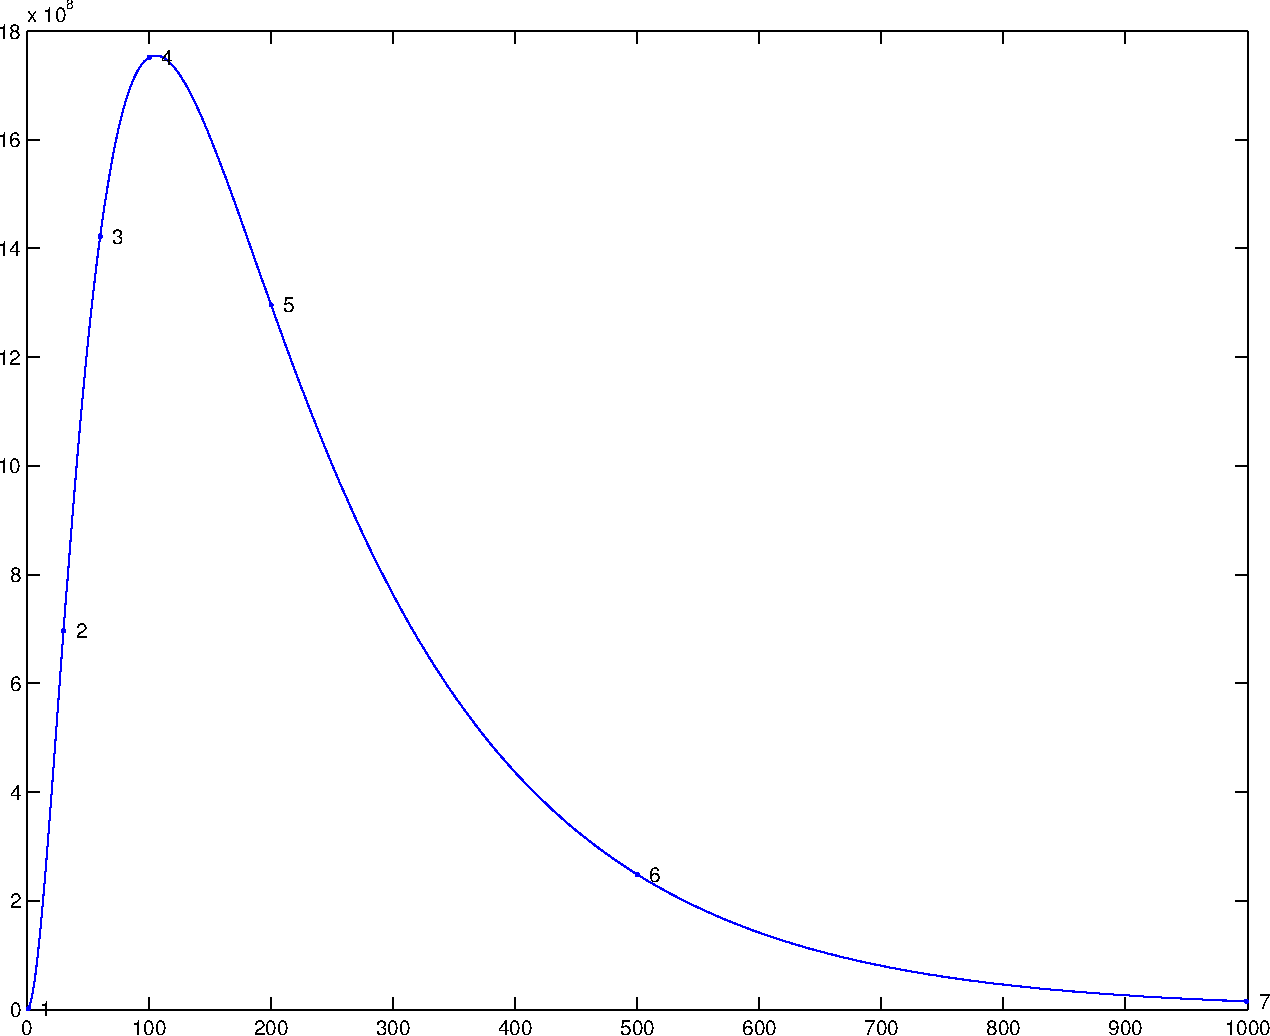
\includegraphics[width=0.5\textwidth]{figures/iss_module/errorplot.pdf}
\caption{Error plot for the ISS-ROF filter using the original image as $u_0$.}\label{fig_iss_errorplot}
\end{figure}

\subsubsection{The difference image}
A quality check is to inspect the difference image. A well tuned ISS filter should only show noise and artifact in the difference image between original and filtered. If you see any structures you know that the filter is modifying the structures in the image. This is an indication that you should try to tweak the parameters a bit more.

\chapter{Command line tool}
KipTool can also be operated from the command line. This is convenient when you want to process many images of the same type or to save memory when you work with large images. The CLI version doesn't have to save the original image for comparison as in the GUI. CLI processing requires that you have a process script file. The typical workflow is that you tune your processing using the GUI and then save the configuration to file. Once you have this file you can start KipTool with
\begin{verbatim}
kiptool -f <configfile.xml>
\end{verbatim}


\chapter{Continued development}
Kiptool is continuously developing to adapt to new challenges at the neutron
imaging beamlines at Paul Scherrer Institut. Unfortunately, it is not only new
development but also bug fixing. To fix bug the input from users is important,
so I kindly ask you to report problems when the software misbehaves.

For the continued development, it also important with feedback regarding
improvements of existing and new features. So, if you have any comments that you
would like to share I appreciate if you send them to me. I cannot promise that I
will implement everything but I will at least consider it.

\bibliographystyle{plain}
\bibliography{../../../doc/references}
%\appendix
%\chapter{License}
%Definitions: The software refers to any revision of MuhRec. The author Anders
%Kaestner is referred to as the author. Any person who installed and intends to
%use or uses the software is referred to as the user.
%\begin{itemize}
%\item The software (source code, binaries, and any supporting material) is the property of the author.
%\item The user is allowed to install and use the software free of charge.
%\item It is not allowed to decompile and/or modify the files in the software distribution.
%\item The software is delivered as is. The author gratefully receives bug
%reports and feature requests but can not promise any updates. In case of updates
%the user will be notified.
%\item The author takes no responsibility for the use of the software and the
%accuracy of the results.
%\item The user is \emph{strongly discouraged} from using the software for
%medical applications.
%\end{itemize}
\end{document}